\documentclass[tikz, border=14pt]{standalone}
\usepackage{tikz}
\usepackage{amsmath,amssymb}
\usepackage{lmodern}
\usepackage[T1]{fontenc}
\usetikzlibrary{
  arrows.meta,
  positioning,
  fit,
  backgrounds,
  calc,
  shapes.geometric,
  decorations.pathreplacing
}

% ── Colour palette ────────────────────────────────────────────────────────────
\definecolor{cbmblue}  {HTML}{1565C0}
\definecolor{cbmbg}    {HTML}{E3F2FD}
\definecolor{cbmborder}{HTML}{1976D2}
\definecolor{nesyred}  {HTML}{C62828}
\definecolor{nesybg}   {HTML}{FFEBEE}
\definecolor{nesyborder}{HTML}{D32F2F}
\definecolor{oodgreen} {HTML}{2E7D32}
\definecolor{oodbg}    {HTML}{E8F5E9}
\definecolor{gatecol}  {HTML}{E65100}
\definecolor{gatebg}   {HTML}{FFF3E0}
\definecolor{sharedcol}{HTML}{37474F}
\definecolor{sharedbg} {HTML}{ECEFF1}
\definecolor{panelbg}  {HTML}{FAFAFA}

% ── Node styles ───────────────────────────────────────────────────────────────
\tikzset{
  % Generic coloured box
  cbox/.style 2 args={
    draw=#1, fill=#2, rounded corners=3.5pt,
    align=center, inner sep=5pt,
    font=\small
  },
  % Standard module box (fixed width)
  modbox/.style={cbox={#1}{#1!9}, text=#1,
    minimum width=3.6cm, minimum height=0.7cm},
  % Wide module box
  wmodbox/.style={cbox={#1}{#1!9}, text=#1,
    minimum width=4.0cm, minimum height=0.7cm},
  % Shared (input / output) box
  sharedmod/.style={cbox={sharedcol}{sharedbg}, text=sharedcol,
    minimum width=9.5cm, minimum height=0.78cm},
  % OOD box
  oodbox/.style={cbox={oodgreen}{oodbg}, text=oodgreen,
    minimum width=3.4cm, minimum height=0.7cm},
  % Alpha-gate box
  gatebox/.style={cbox={gatecol}{gatebg}, text=gatecol,
    minimum width=4.0cm, minimum height=0.78cm},
  % Tiny concept / rule square
  csq/.style={draw=cbmblue, fill=cbmbg,
    minimum width=0.28cm, minimum height=0.28cm, inner sep=0pt},
  rsq/.style={draw=nesyred, fill=nesybg,
    minimum width=0.28cm, minimum height=0.28cm, inner sep=0pt},
  % Arrow styles
  arr/.style  ={-{Stealth[length=5pt,width=3.5pt]}, line width=0.9pt, color=#1},
  darr/.style ={-{Stealth[length=5pt,width=3.5pt]}, line width=0.9pt,
                dashed, color=#1},
  % Annotation label
  annot/.style={font=\scriptsize\itshape, text=gray!70!black, align=center},
}

% ─────────────────────────────────────────────────────────────────────────────
\begin{document}
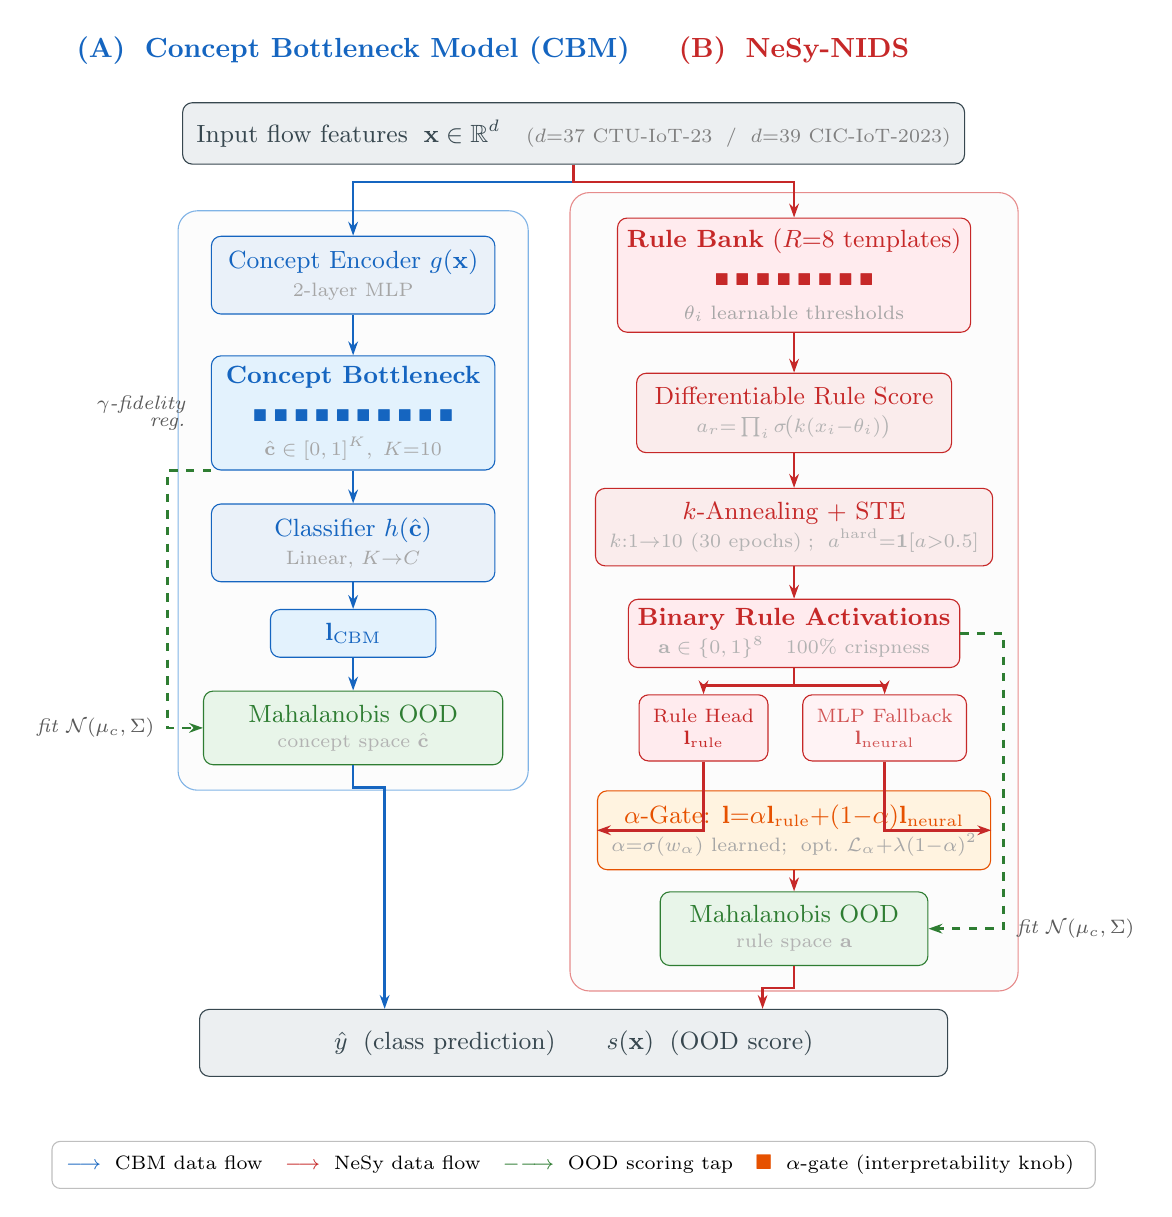
\begin{tikzpicture}

% ============================================================
% COORDINATES  (all explicit for predictable layout)
% Left column (CBM):  x = -2.8
% Right column (NeSy): x =  2.8
% Centre:              x =  0
% ============================================================

% ── INPUT ─────────────────────────────────────────────────────────────────────
\node[sharedmod] (input) at (0, 0)
  {Input flow features\; $\mathbf{x} \in \mathbb{R}^{d}$\quad
   \textcolor{gray}{\scriptsize($d{=}37$ CTU-IoT-23 \;/\; $d{=}39$ CIC-IoT-2023)}};

% ── CBM ENCODER ───────────────────────────────────────────────────────────────
\node[modbox=cbmblue] (cbm_enc) at (-2.8, -1.8)
  {Concept Encoder $g(\mathbf{x})$\\[-1pt]
   \textcolor{gray!70}{\scriptsize 2-layer MLP}};

% ── CONCEPT BOTTLENECK ────────────────────────────────────────────────────────
\node[draw=cbmblue, fill=cbmbg, rounded corners=3.5pt,
      minimum width=3.6cm, minimum height=1.45cm,
      align=center, font=\small, text=cbmblue] (cbm_bottle) at (-2.8, -3.55)
  {\textbf{Concept Bottleneck}\\[3pt]
   {\tiny\textcolor{cbmblue}{%
     $\blacksquare\;\blacksquare\;\blacksquare\;\blacksquare\;\blacksquare\;%
      \blacksquare\;\blacksquare\;\blacksquare\;\blacksquare\;\blacksquare$}}\\[1pt]
   \textcolor{gray!70}{\scriptsize $\hat{\mathbf{c}}\in[0,1]^{K},\; K{=}10$}};

% Gamma annotation — inside CBM panel, left of bottleneck
\node[annot, left=0.2cm of cbm_bottle, text width=1.3cm, align=right]
  {$\gamma$-fidelity\\[-2pt]reg.};

% ── CBM CLASSIFIER ────────────────────────────────────────────────────────────
\node[modbox=cbmblue] (cbm_head) at (-2.8, -5.2)
  {Classifier $h(\hat{\mathbf{c}})$\\[-1pt]
   \textcolor{gray!70}{\scriptsize Linear, $K{\to}C$}};

% CBM logits output
\node[cbox={cbmblue}{cbmbg}, text=cbmblue,
      minimum width=2.1cm, minimum height=0.6cm,
      font=\small] (cbm_logits) at (-2.8, -6.35)
  {$\mathbf{l}_{\mathrm{CBM}}$};

% ── OOD CBM ───────────────────────────────────────────────────────────────────
\node[oodbox, minimum width=3.8cm] (ood_cbm) at (-2.8, -7.55)
  {Mahalanobis OOD\\[-2pt]
   \textcolor{gray!60}{\scriptsize concept space $\hat{\mathbf{c}}$}};

% ============================================================
% NeSy-NIDS  (right column)
% ============================================================

% ── RULE BANK ─────────────────────────────────────────────────────────────────
\node[draw=nesyred, fill=nesybg, rounded corners=3.5pt,
      minimum width=4.0cm, minimum height=1.45cm,
      align=center, font=\small, text=nesyred] (rule_bank) at (2.8, -1.8)
  {\textbf{Rule Bank} ($R{=}8$ templates)\\[3pt]
   {\tiny\textcolor{nesyred}{%
     $\blacksquare\;\blacksquare\;\blacksquare\;\blacksquare\;%
      \blacksquare\;\blacksquare\;\blacksquare\;\blacksquare$}}\\[1pt]
   \textcolor{gray!70}{\scriptsize $\theta_i$ learnable thresholds}};

% ── DIFFERENTIABLE SCORING ────────────────────────────────────────────────────
\node[wmodbox=nesyred] (diff_score) at (2.8, -3.55)
  {Differentiable Rule Score\\[-1pt]
   \textcolor{gray!60}{\scriptsize
   $a_r{=}\prod_i \sigma\!\bigl(k(x_i{-}\theta_i)\bigr)$}};

% ── k-ANNEALING + STE ─────────────────────────────────────────────────────────
\node[wmodbox=nesyred] (ste_box) at (2.8, -5.0)
  {$k$-Annealing + STE\\[-1pt]
   \textcolor{gray!60}{\scriptsize
   $k{:}1{\to}10$ (30 epochs)\;;\;
   $a^{\mathrm{hard}}{=}\mathbf{1}[a{>}0.5]$}};

% ── BINARY RULE ACTIVATIONS ───────────────────────────────────────────────────
\node[draw=nesyred, fill=nesybg, rounded corners=3.5pt,
      minimum width=4.0cm, minimum height=0.75cm,
      align=center, font=\small, text=nesyred] (rule_act) at (2.8, -6.35)
  {\textbf{Binary Rule Activations}\\[-1pt]
   \textcolor{gray!60}{\scriptsize $\mathbf{a}\in\{0,1\}^{8}$\quad
   100\% crispness}};

% ── RULE HEAD + MLP FALLBACK ──────────────────────────────────────────────────
\node[cbox={nesyred}{nesybg}, text=nesyred,
      minimum width=1.6cm, minimum height=0.6cm,
      font=\scriptsize] (rule_head) at (1.65, -7.55)
  {Rule Head\\$\mathbf{l}_{\mathrm{rule}}$};

\node[cbox={nesyred}{nesybg!60!white}, text=nesyred!80,
      minimum width=1.6cm, minimum height=0.6cm,
      font=\scriptsize] (mlp_fb) at (3.95, -7.55)
  {MLP Fallback\\$\mathbf{l}_{\mathrm{neural}}$};

% ── ALPHA GATE ────────────────────────────────────────────────────────────────
\node[gatebox] (alpha_gate) at (2.8, -8.85)
  {$\alpha$-Gate: $\mathbf{l}{=}\alpha\mathbf{l}_{\mathrm{rule}}{+}(1{-}\alpha)\mathbf{l}_{\mathrm{neural}}$\\[-1pt]
   \textcolor{gray!70}{\scriptsize $\alpha{=}\sigma(w_\alpha)$ learned;\;
   opt.\ $\mathcal{L}_\alpha{+}\lambda(1{-}\alpha)^2$}};

% ── OOD NeSy ──────────────────────────────────────────────────────────────────
\node[oodbox] (ood_nesy) at (2.8, -10.1)
  {Mahalanobis OOD\\[-2pt]
   \textcolor{gray!60}{\scriptsize rule space $\mathbf{a}$}};

% ── OUTPUT ────────────────────────────────────────────────────────────────────
\node[sharedmod, minimum height=0.85cm] (output) at (0, -11.55)
  {$\hat{y}$\; (class prediction)\qquad
   $s(\mathbf{x})$\; (OOD score)};

% ============================================================
% ARROWS
% ============================================================

% Input → CBM encoder
\draw[arr=cbmblue]
  (input.south) -- ++(0,-0.22) -| (cbm_enc.north);

% Input → Rule bank
\draw[arr=nesyred]
  (input.south) -- ++(0,-0.22) -| (rule_bank.north);

% CBM chain
\draw[arr=cbmblue] (cbm_enc.south) -- (cbm_bottle.north);
\draw[arr=cbmblue] (cbm_bottle.south) -- (cbm_head.north);
\draw[arr=cbmblue] (cbm_head.south) -- (cbm_logits.north);
\draw[arr=cbmblue] (cbm_logits.south) -- (ood_cbm.north);

% NeSy chain
\draw[arr=nesyred] (rule_bank.south) -- (diff_score.north);
\draw[arr=nesyred] (diff_score.south) -- (ste_box.north);
\draw[arr=nesyred] (ste_box.south)    -- (rule_act.north);
\draw[arr=nesyred] (rule_act.south) -- ++(0,-0.22)
  -| (rule_head.north);
\draw[arr=nesyred] (rule_act.south) -- ++(0,-0.22)
  -| (mlp_fb.north);
\draw[arr=nesyred] (rule_head.south) |- (alpha_gate.west);
\draw[arr=nesyred] (mlp_fb.south)    |- (alpha_gate.east);
\draw[arr=nesyred] (alpha_gate.south) -- (ood_nesy.north);

% OOD concept space: dashed tap from concept bottleneck
\draw[darr=oodgreen]
  (cbm_bottle.south west) -- ++(-0.55, 0)
  |- node[annot, left=1pt, midway] {fit $\mathcal{N}(\mu_c,\Sigma)$} (ood_cbm.west);

% OOD rule space: dashed tap from rule activations
\draw[darr=oodgreen]
  (rule_act.east) -- ++(0.55, 0)
  |- node[annot, right=1pt, midway] {fit $\mathcal{N}(\mu_c,\Sigma)$} (ood_nesy.east);

% CBM logits → output
\draw[arr=cbmblue]
  (ood_cbm.south) -- ++(0,-0.28)
  -| ([xshift=-2.4cm]output.north);

% NeSy → output
\draw[arr=nesyred]
  (ood_nesy.south) -- ++(0,-0.28)
  -| ([xshift=2.4cm]output.north);

% ============================================================
% BACKGROUND PANELS
% ============================================================
\begin{scope}[on background layer]
  % CBM panel
  \node[draw=cbmborder, fill=panelbg, rounded corners=7pt,
        fit=(cbm_enc)(cbm_bottle)(cbm_head)(cbm_logits)(ood_cbm),
        inner sep=9pt, opacity=0.55] (cbm_panel) {};
  % NeSy panel
  \node[draw=nesyborder, fill=panelbg, rounded corners=7pt,
        fit=(rule_bank)(diff_score)(ste_box)(rule_act)
            (rule_head)(mlp_fb)(alpha_gate)(ood_nesy),
        inner sep=9pt, opacity=0.55] (nesy_panel) {};
\end{scope}

% Panel headings — placed at fixed y above panels, avoiding the input node
\node[font=\normalsize\bfseries, text=cbmblue]
  at (-2.8, 1.05) {(A)\; Concept Bottleneck Model (CBM)};
\node[font=\normalsize\bfseries, text=nesyred]
  at (2.8,  1.05) {(B)\; NeSy-NIDS};

% ── LEGEND ── placed below output box, centred ───────────────────────────────
\node[draw=gray!50, fill=white, rounded corners=3pt,
      align=left, font=\scriptsize,
      inner sep=5pt] (legend) at (0, -13.1) {
  \textcolor{cbmblue}{$\longrightarrow$}\; CBM data flow\quad
  \textcolor{nesyred}{$\longrightarrow$}\; NeSy data flow\quad
  \textcolor{oodgreen}{$--\!\!\!\rightarrow$}\; OOD scoring tap\quad
  \textcolor{gatecol}{$\blacksquare$}\; $\alpha$-gate (interpretability knob)
};

\end{tikzpicture}
\end{document}
